\chapter{Лекция 9. Двудольные графы. Паросочетания. Задача о максимальном потоке}

% ============================================================
% ДВУДОЛЬНЫЕ ГРАФЫ
% ============================================================

\subsection*{Двудольные графы}

\begin{defn}{Двудольный граф}{bipartite}
$G(V, E)$ --- \textbf{двудольный}:

$V = V_1 \sqcup V_2$ т.\,ч. $\forall\, e \in E$: $u \in V_1$, $v \in V_2$
\quad (начальная вершина --- любая).
\end{defn}

\medskip
\noindent\textbf{Примеры} (доля $V_1$ --- синяя, доля $V_2$ --- оранжевая):

% Пример 1: дерево (11 вершин) — двудольный
% Граф: p21-example-1.graph
\grfig{figures/p21-example-1.pdf}{Двудольный: дерево 11 вершин}
\noindent\textit{Пример 1.} Любое дерево двудольно: раскрашиваем вершины
по чётности уровня. Здесь $V_1 = \{1, 3, 4, 6, 9, 11\}$ (чётные уровни),
$V_2 = \{2, 5, 7, 8, 10\}$ (нечётные) --- каждое ребро соединяет
соседние уровни, т.\,е. разные доли.

% Пример 2: решётка/сетка (10 вершин) — двудольный
% Граф: p21-example-2.graph
\grfig{figures/p21-example-2.pdf}{Двудольный: решётка 10 вершин}
\noindent\textit{Пример 2.} Решётка двудольна (<<шахматная>> раскраска):
$V_1 = \{1, 3, 6, 8, 9\}$, $V_2 = \{2, 4, 5, 7, 10\}$ --- у каждого
ребра концы разного цвета.

% Пример 3: треугольник (3 вершины) — НЕ двудольный
% Граф: p21-example-3.graph
\grfig{figures/p21-example-3.pdf}{НЕ двудольный: треугольник}
\noindent\textit{Пример 3.} Треугольник \emph{не} двудолен: положив
$1 \in V_1$, получаем $2 \in V_2$, $3 \in V_1$ --- но тогда ребро
$3$--$1$ (красное) соединяет две вершины одной доли. Куда ни относи
вершины, одно ребро всегда останется внутри доли.

\begin{statement}{Критерий двудольности графа}{bipartite-criterion}
$G$ --- двудольный $\;\Leftrightarrow\;$ $G$ не содержит циклов нечётной длины.
\end{statement}

\begin{proof}
\textbf{($\Rightarrow$) Если граф двудолен, нечётных циклов нет.} Пусть
$V=V_1\sqcup V_2$ --- доли, и все рёбра идут между ними. Любой цикл
$v_0\,v_1\,\dots\,v_k\,v_0$ при движении по рёбрам поочерёдно меняет долю:
$v_0\in V_1\Rightarrow v_1\in V_2\Rightarrow v_2\in V_1$ и так далее. Чтобы
вернуться в исходную долю (в вершину $v_0$), число шагов должно быть чётным,
поэтому длина любого цикла чётна --- нечётных циклов нет.

\smallskip
\textbf{($\Leftarrow$) Если нечётных циклов нет, граф двудолен.} Достаточно
доказать утверждение для каждой связной компоненты по отдельности. Зафиксируем
в компоненте вершину $s$ и для каждой вершины $v$ рассмотрим расстояние
$d(s,v)$ (длину кратчайшего пути, BFS-нумерация). Положим
\[
  V_1=\{v\colon d(s,v)\text{ чётно}\},\qquad
  V_2=\{v\colon d(s,v)\text{ нечётно}\}.
\]
Покажем, что любое ребро $uv$ соединяет вершины из разных долей. Предположим
противное: пусть $u,v$ лежат в одной доле, то есть $d(s,u)$ и $d(s,v)$ одной
чётности. Рассмотрим замкнутый маршрут: кратчайший путь $s\to u$, ребро $uv$ и
кратчайший путь $v\to s$. Его длина равна $d(s,u)+1+d(s,v)$ --- сумма двух
чисел одной чётности плюс единица, то есть \emph{нечётна}. Замкнутый маршрут
нечётной длины обязательно содержит простой цикл нечётной длины, что
противоречит условию. Значит концы каждого ребра попадают в разные доли, и
разбиение $V=V_1\sqcup V_2$ задаёт двудольность.

\smallskip
\textit{Иллюстрация.} Цикл \emph{чётной} длины ($C_8$ слева)
раскрашивается чередованием $V_1,V_2,V_1,V_2,\dots$ --- двудолен. В цикле
\emph{нечётной} длины ($C_7$ справа) при таком чередовании последняя
вершина оказывается смежной с первой вершиной той же доли (красное
ребро) --- разбить на две доли невозможно.

\grfig[0.45]{figures/p21-example-4.pdf}{Критерий: чётный цикл $C_8$ (двудольный)}
\grfig[0.45]{figures/p21-example-5.pdf}{Критерий: нечётный цикл $C_7$ (не двудольный)}

\end{proof}

% ============================================================
% ПАРОСОЧЕТАНИЯ
% ============================================================

\subsection*{Паросочетания}

\begin{defn}{Паросочетание}{matching}
$G(V, E)$ --- двудольный, $V = V_1 \sqcup V_2$.

\textbf{Паросочетание} для $G$: $\hat{E} \subseteq E$ т.\,ч. $\forall\, e_i, e_j \in \hat{E}$
--- инцидентны не более чем одной общей вершине
(т.\,е. рёбра паросочетания попарно не имеют общих вершин).
\end{defn}

\begin{defn}{Максимальное паросочетание}{max-matching}
\textbf{Максимальное паросочетание} --- максимальное по включению:
к нему нельзя добавить ни одно ребро графа, не нарушив определение.
\end{defn}

\begin{defn}{Наибольшее паросочетание}{maximum-matching}
\textbf{Наибольшее паросочетание} --- наибольшее количество рёбер для данного графа.
\end{defn}

\medskip
\noindent\textbf{Примеры.} Один и тот же граф --- цепь $1$--$2$--$3$--$4$;
рёбра паросочетания --- зелёные жирные, насыщенные ими вершины ---
закрашены:

% Пример 1: {1-2} — не макс, не наиб.
% Граф: p22-example-1.graph
\grfig[0.4]{figures/p22-example-1.pdf}{Паросочетание $\{1\text{--}2\}$: не макс., не наиб.}
\noindent\textit{Пример 1.} $\hat E = \{1\text{--}2\}$ --- \textbf{не
максимальное}: можно добавить ребро $3$--$4$ (его концы свободны);
значит, и \textbf{не наибольшее}.

% Пример 2: {2-3} — макс., не наиб.
% Граф: p22-example-2.graph
\grfig[0.4]{figures/p22-example-2.pdf}{Паросочетание $\{2\text{--}3\}$: макс., но не наиб.}
\noindent\textit{Пример 2.} $\hat E = \{2\text{--}3\}$ ---
\textbf{максимальное}: оба оставшихся ребра ($1$--$2$ и $3$--$4$)
задевают занятые вершины $2$ и $3$, добавить нечего. Но \textbf{не
наибольшее}: в примере~3 есть паросочетание из двух рёбер.

% Пример 3: {1-2, 3-4} — макс. и наиб.
% Граф: p22-example-3.graph
\grfig[0.4]{figures/p22-example-3.pdf}{Паросочетание $\{1\text{--}2,\ 3\text{--}4\}$: макс. и наиб.}
\noindent\textit{Пример 3.} $\hat E = \{1\text{--}2,\ 3\text{--}4\}$ ---
\textbf{максимальное и наибольшее}: все 4 вершины насыщены, больше двух
непересекающихся рёбер в графе из 4 вершин быть не может.

% Пример 4: {3-4} — не макс., не наиб.
% Граф: p22-example-4.graph
\grfig[0.4]{figures/p22-example-4.pdf}{Паросочетание $\{3\text{--}4\}$: не макс., не наиб.}
\noindent\textit{Пример 4.} $\hat E = \{3\text{--}4\}$ --- симметричный
к примеру~1 случай: можно добавить ребро $1$--$2$, поэтому паросочетание
\textbf{не максимальное} (и не наибольшее).

\medskip
\textbf{NB:} $\max |\hat E| \leq \min(|V_1|, |V_2|)$ --- каждое ребро
паросочетания занимает по одной вершине в каждой доле, поэтому рёбер не
больше, чем вершин в меньшей доле.

\medskip
\textbf{Упр.} Доказать, что:
\begin{itemize}
  \item наибольшее $\Rightarrow$ максимальное;
  \item максимальное $\not\Rightarrow$ наибольшее.
\end{itemize}

\textit{Решение.} Если бы наибольшее паросочетание не было максимальным,
к нему можно было бы добавить ребро и получить паросочетание большего
размера --- противоречие с <<наибольшестью>>. Обратная импликация
неверна: контрпример --- примеры 2 и 3 выше ($\{2\text{--}3\}$
максимально, но меньше наибольшего).

\medskip
\textbf{Упр.} Пример $G$ с наибольшим паросочетанием $\hat{E}$, т.\,ч. $|\hat{E}| < \min(|V_1|, |V_2|)$.

\textit{Решение.} <<Звезда>>: $V_1 = \{a, b\}$, $V_2 = \{x, y\}$, рёбра
$a$--$x$, $a$--$y$. Все рёбра проходят через $a$, поэтому любое
паросочетание содержит не более одного ребра: $|\hat E| = 1 <
2 = \min(|V_1|, |V_2|)$.

% ============================================================
% АЛГОРИТМ НАХОЖДЕНИЯ НАИБОЛЬШЕГО ПАРОСОЧЕТАНИЯ
% ============================================================

\begin{algo}{Алгоритм поиска наибольшего паросочетания}{matching-algo}
\textbf{Дано:} $G(V, E)$ --- двудольный, $V = V_1 \sqcup V_2$.

\textbf{Найти:} наибольшее паросочетание $\hat{E}$.

\medskip
\textbf{Инициализация.} Добавляем фиктивные вершины $S$ и $F$:
\[
  \forall\, v_i \in V_1\colon\ \text{дуга } S \to v_i;
  \qquad
  \forall\, w_j \in V_2\colon\ \text{дуга } w_j \to F,
\]
а все рёбра графа ориентируем слева направо: $v_i \to w_j$.

\medskip
\textbf{Step.} Пока существует путь $l\colon S \to \ldots \to F$:
\begin{enumerate}
  \item находим такой путь (любым обходом);
  \item \emph{инвертируем} на нём все рёбра между долями:
        пройденное ребро $v_i \to w_j$ разворачивается в $w_j \to v_i$
        --- развёрнутые рёбра и есть текущее паросочетание;
  \item крайние дуги пути ($S \to v_i$ и $w_j \to F$) удаляем ---
        вершины $v_i$ и $w_j$ насыщены.
\end{enumerate}
Когда путей из $S$ в $F$ больше нет, развёрнутые рёбра $w_j \to v_i$
образуют наибольшее паросочетание.

\medskip
\textit{Почему это работает:} путь $S \to v_i \to w_j \to v_k \to \ldots
\to F$, проходящий по развёрнутому ребру $w_j \to v_k$, --- это
\emph{увеличивающий путь}: он отбирает $w_j$ у вершины $v_k$ и тут же
находит ей новую пару, а в конце насыщает одну новую вершину каждой
доли. Число рёбер паросочетания каждый раз растёт на $1$.

\medskip
\noindent\textbf{Пример.} $V_1 = \{A, B, C, D\}$,
$V_2 = \{\alpha, \beta, \gamma\}$, рёбра:
$A\alpha$, $A\beta$, $B\alpha$, $B\beta$, $C\beta$, $C\gamma$,
$D\alpha$, $D\gamma$.

% Граф: p22-example-5.graph
\grfig[0.5]{figures/p22-example-5.pdf}{Алг. наиб. паросочетания: $S$, доли $\{A,B,C,D\}$ и $\{\alpha,\beta,\gamma\}$, $F$}

Находим пути и инвертируем (стрелки <<туда-обратно>>):
\begin{enumerate}
  \item $S, B, \beta, F$ --- ребро $B\beta$ разворачивается:
        $\beta \to B$; паросочетание $\{B\beta\}$;
  \item $S, C, \beta, B, \alpha, F$ --- путь идёт по развёрнутому ребру
        $\beta \to B$ (отбираем $\beta$ у $B$): теперь $\beta \to C$,
        $\alpha \to B$; паросочетание $\{C\beta, B\alpha\}$;
  \item $S, A, \beta, C, \gamma, F$ --- аналогично $\beta$ переходит к
        $A$, а $C$ получает $\gamma$;
        паросочетание $\{A\beta, B\alpha, C\gamma\}$.
\end{enumerate}

\textbf{Итог:} наибольшее паросочетание
$\hat E = \{A\beta,\; B\alpha,\; C\gamma\}$, $|\hat E| = 3 =
\min(|V_1|, |V_2|)$ --- вершина $D$ осталась свободной.

\medskip
\noindent\textbf{Работа алгоритма по шагам} (текущий путь --- оранжевый,
развёрнутые рёбра паросочетания --- зелёные, удалённые дуги --- бледные):

\begin{center}\begin{tabular}{cc}
\shortstack{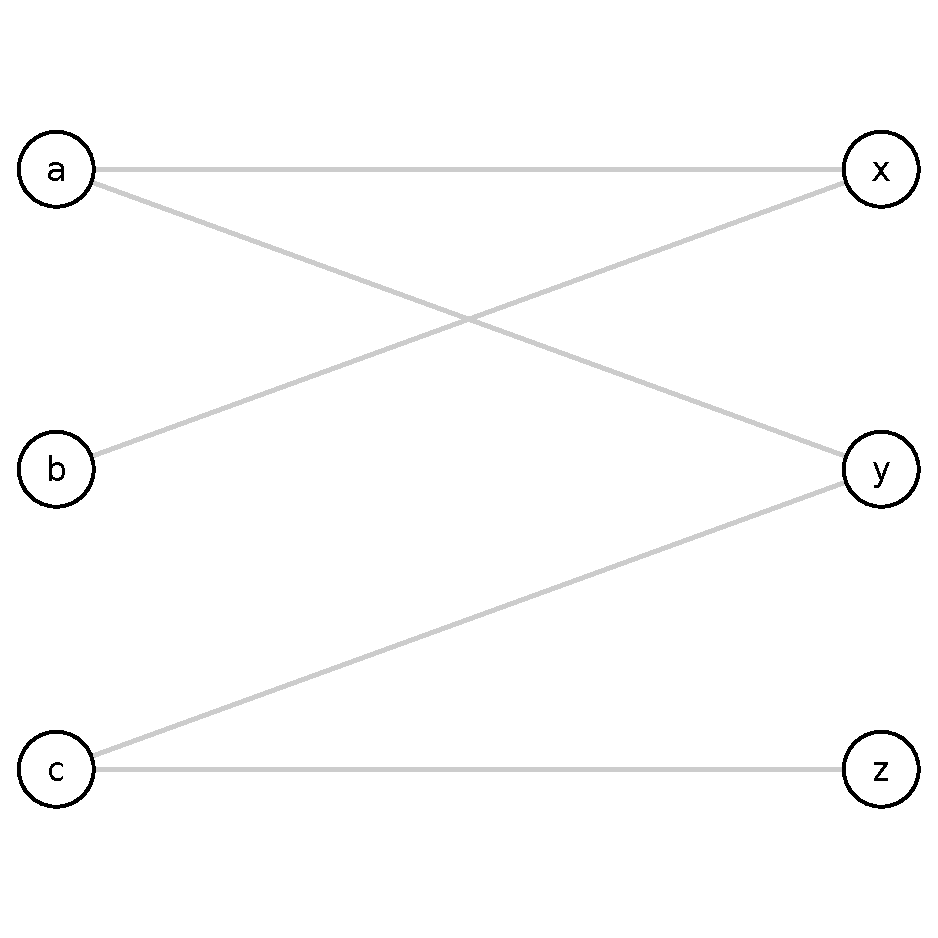
\includegraphics[width=0.46\textwidth]{python/lec09/matching/matching-0.pdf}\\[2pt]{\scriptsize Шаг 0. Сеть с фиктивными $S$ и $F$}} &
\shortstack{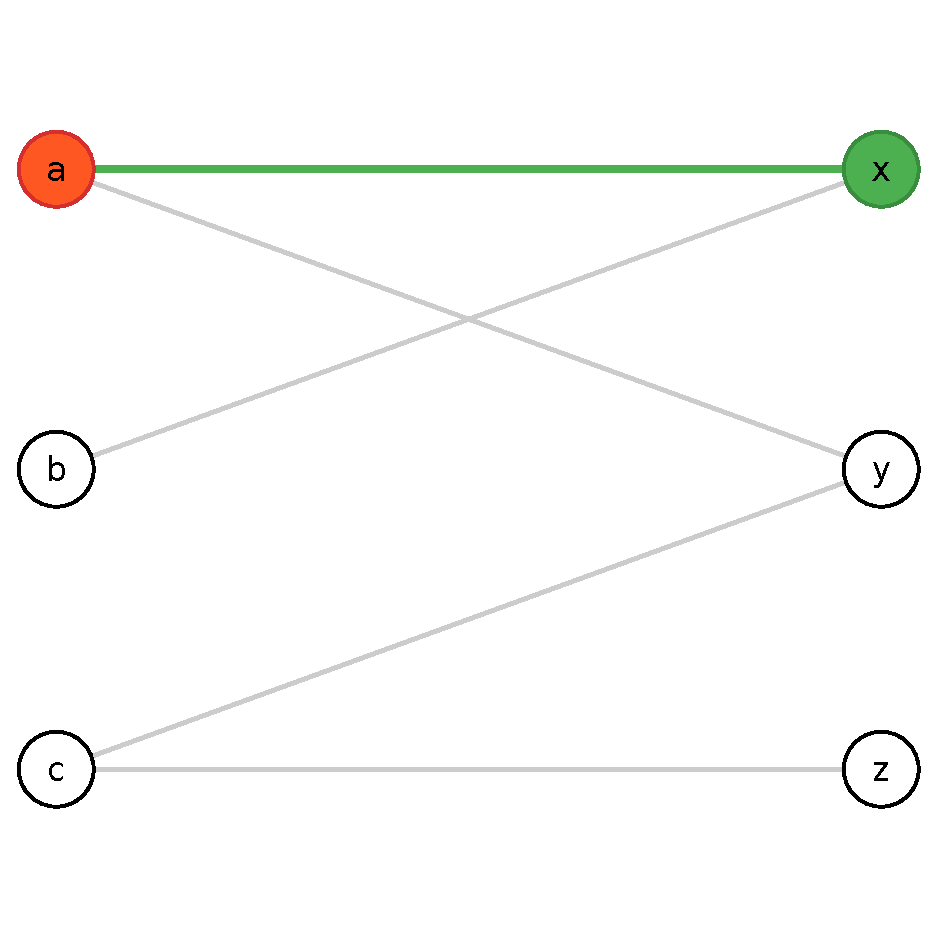
\includegraphics[width=0.46\textwidth]{python/lec09/matching/matching-1.pdf}\\[2pt]{\scriptsize Шаг 1. Путь 1: $S, B, \beta, F$}} \\
\end{tabular}\end{center}
\begin{center}\begin{tabular}{cc}
\shortstack{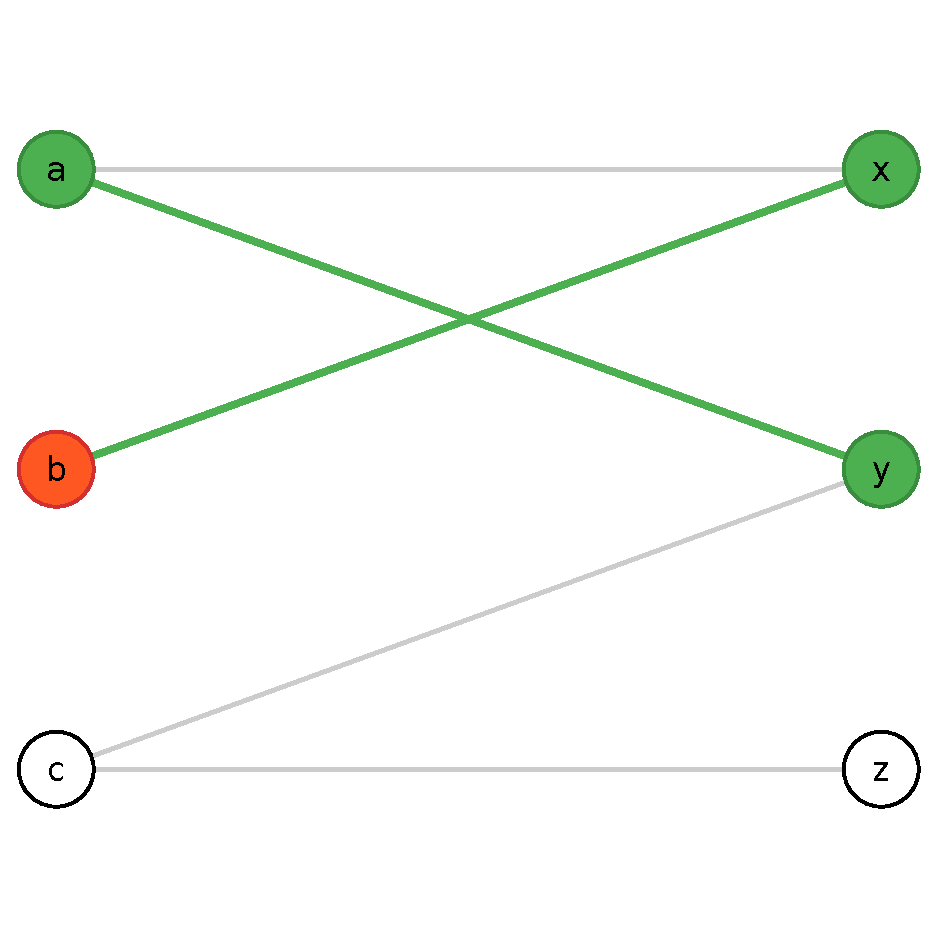
\includegraphics[width=0.46\textwidth]{python/lec09/matching/matching-2.pdf}\\[2pt]{\scriptsize Шаг 2. $B\beta$ развёрнуто: $\{B\beta\}$}} &
\shortstack{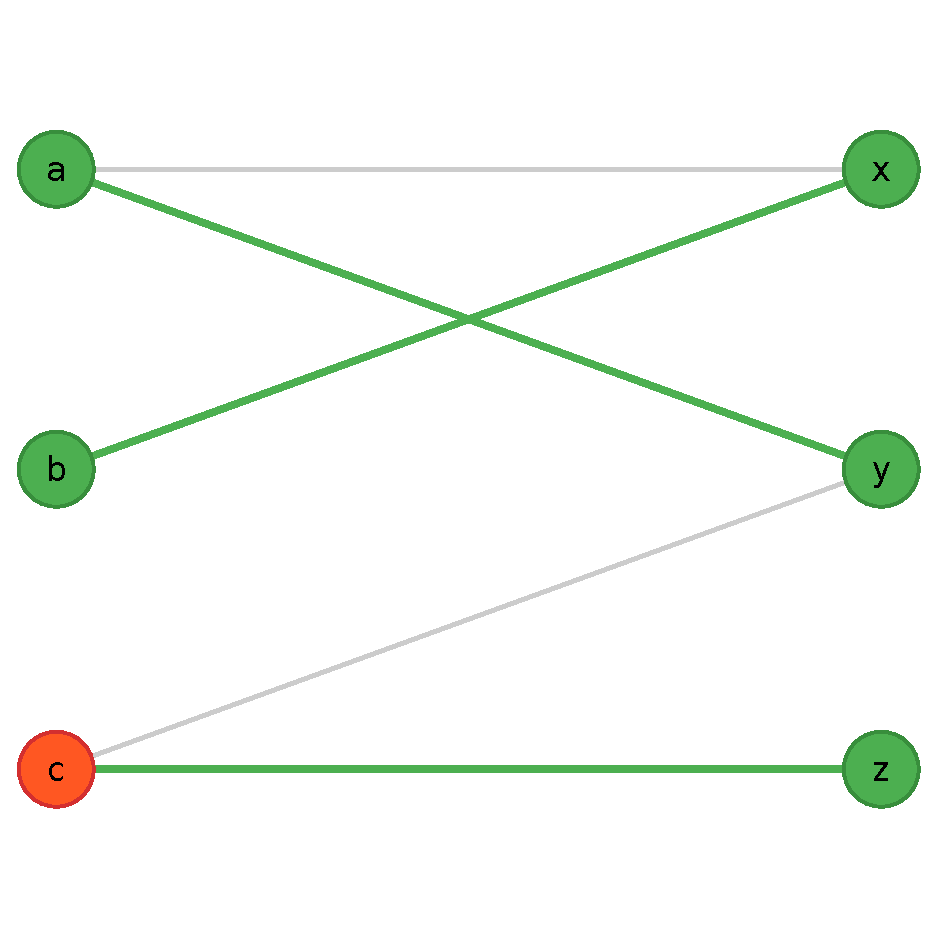
\includegraphics[width=0.46\textwidth]{python/lec09/matching/matching-3.pdf}\\[2pt]{\scriptsize Шаг 3. Путь 2: $S, C, \beta, B, \alpha, F$}} \\
\end{tabular}\end{center}
\begin{center}\begin{tabular}{cc}
\shortstack{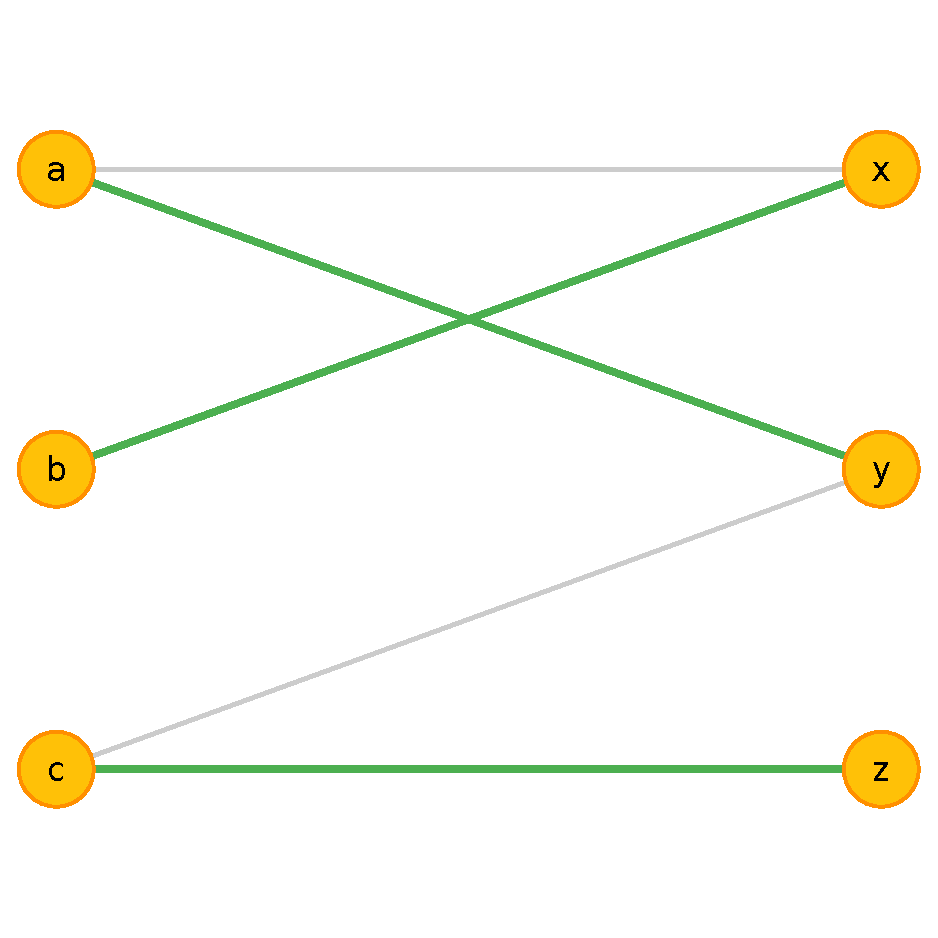
\includegraphics[width=0.46\textwidth]{python/lec09/matching/matching-4.pdf}\\[2pt]{\scriptsize Шаг 4. $\beta$ перешла к $C$, $B$ получил $\alpha$}} &
\shortstack{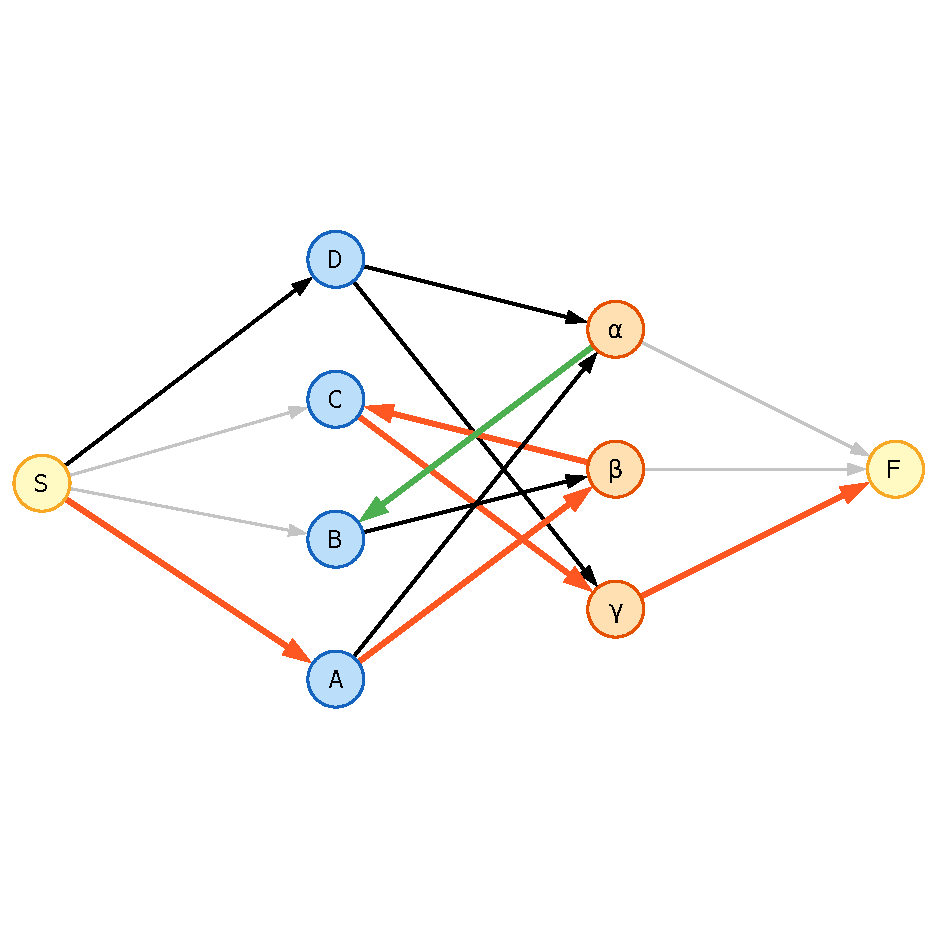
\includegraphics[width=0.46\textwidth]{python/lec09/matching/matching-5.pdf}\\[2pt]{\scriptsize Шаг 5. Путь 3: $S, A, \beta, C, \gamma, F$}} \\
\end{tabular}\end{center}
\begin{center}
\shortstack{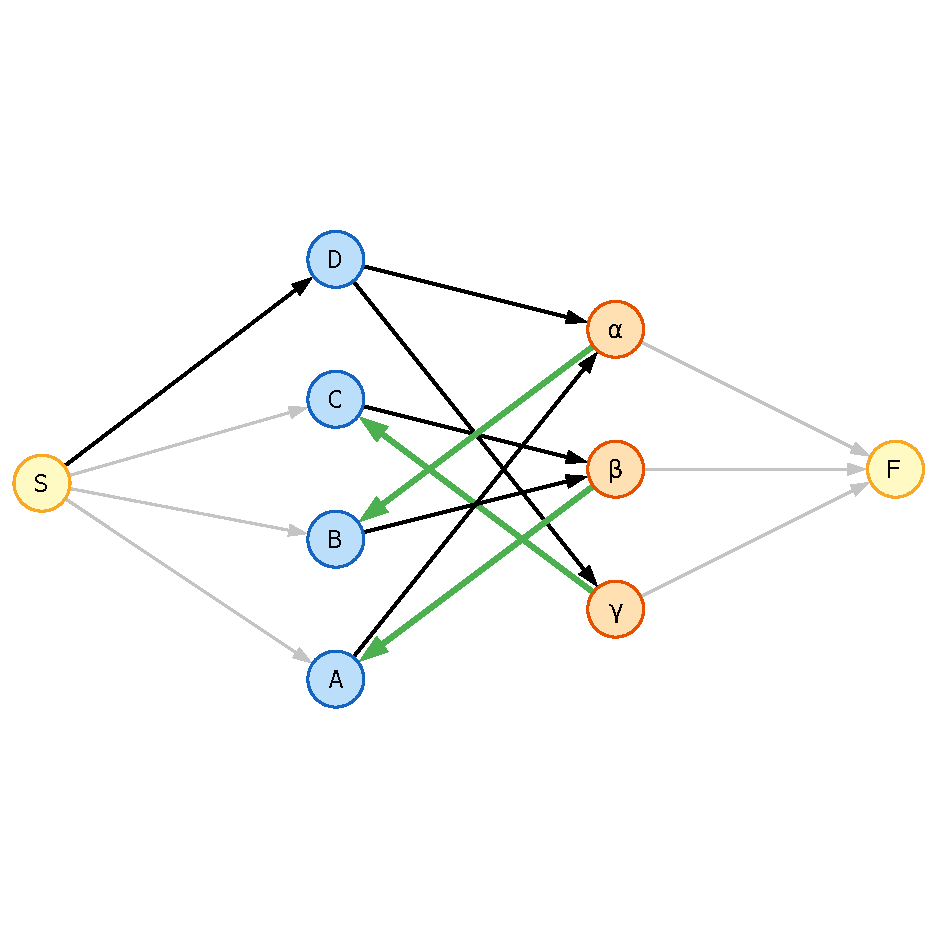
\includegraphics[width=0.5\textwidth]{python/lec09/matching/matching-6.pdf}\\[2pt]{\scriptsize Шаг 6. Итог: $\{A\beta, B\alpha, C\gamma\}$, путей $S \to F$ больше нет}}
\end{center}

\medskip
\textbf{Упр.} Почему паросочетание наибольшее?

\textit{Ответ (идея, лемма Бержа).} Паросочетание наибольшее
$\Leftrightarrow$ для него нет увеличивающего пути (чередующегося пути
между двумя свободными вершинами). Алгоритм останавливается ровно тогда,
когда пути $S \to F$ нет, т.\,е. нет и увеличивающего пути. Если бы
существовало паросочетание $\hat E'$ с $|\hat E'| > |\hat E|$, то в
симметрической разности $\hat E \,\Delta\, \hat E'$ (каждая вершина
задета не более чем двумя рёбрами --- это набор путей и чётных циклов)
нашлась бы компонента-путь, где рёбер $\hat E'$ больше, чем рёбер
$\hat E$, --- это и есть увеличивающий путь для $\hat E$. Противоречие.
\end{algo}

% ============================================================
% ЗАДАЧА О МАКСИМАЛЬНОМ ПОТОКЕ В СЕТИ
% ============================================================

\subsection*{Задача о максимальном потоке в сети}

\begin{defn}{Сеть}{network}
$G(V, E)$ --- \textbf{сеть}: \quad (орграф)
\begin{itemize}
  \item \textbf{исток:} $S$ --- нет входящих рёбер!
  \item \textbf{сток/устье:} $F$ --- нет исходящих рёбер!
\end{itemize}

$\sigma\colon E \to \mathbb{R}_{\geq 0}$ \quad (пропускная способность, пока на рёбрах).
\end{defn}

\begin{defn}{Поток}{flow}
\textbf{Поток:} $f\colon E \to \mathbb{R}$, свойства:
\begin{enumerate}
  \item $0 \leq f(e) \leq \sigma(e)$
  \item \textbf{Условие балансировки:}
        $\forall\, v \in V \setminus \{S, F\}$:\;
        $\displaystyle\sum_{\substack{e\colon u \to v \\ u \in V}} f(e) = 
         \displaystyle\sum_{\substack{e\colon v \to w \\ w \in V}} f(e)$

        \quad (поток входящий = поток исходящий)
\end{enumerate}
\end{defn}

\begin{defn}{Мощность потока}{flow-value}
\textbf{Мощность потока} $|f|$ = суммарное количество перемещаемого в единицу времени
(всё, что вытекает из $S$).

$|f| \to \max$

\textbf{Поток --- функция, НЕ число!}
\end{defn}

\medskip
\exhead{Пример.} Сеть с пропускными способностями (подпись ребра ---
$f/\sigma$, т.\,е. <<поток / пропускная способность>>):

\begin{center}
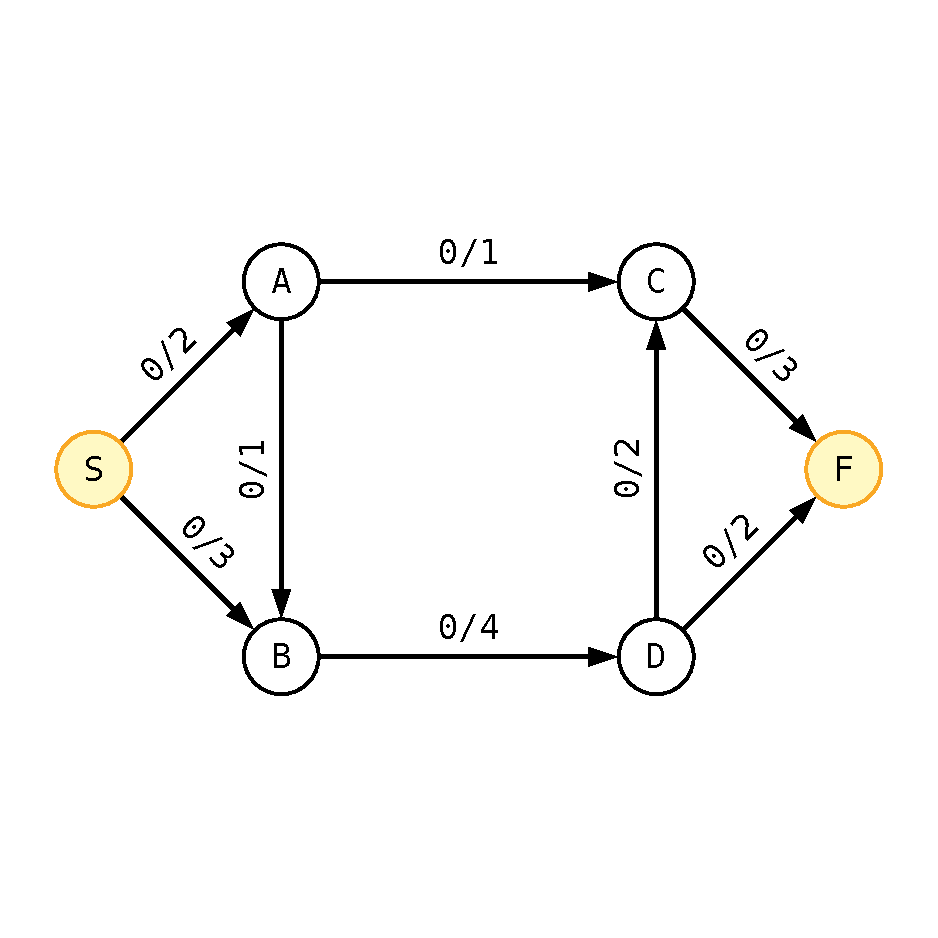
\includegraphics[width=0.5\textwidth]{python/lec09/flowexample/flowex-0.pdf}
\end{center}

Ищем пути из $S$ в $F$ и пускаем по каждому максимум возможного ---
\emph{минимум остаточных пропускных способностей рёбер пути} (самое
<<узкое горлышко>> пути ограничивает весь путь):

\begin{enumerate}
  \item путь $S, B, D, F$: остатки рёбер $3, 4, 2$, узкое место ---
        $DF$, $\min = 2$ --- пускаем $2$;
  \item путь $S, A, C, F$: остатки $2, 1, 3$, узкое место $AC$,
        $\min = 1$ --- пускаем $1$;
  \item путь $S, A, B, D, C, F$: остатки $1, 1, 2, 2, 2$, $\min = 1$
        --- пускаем $1$;
  \item путь $S, B, D, C, F$: остатки $1, 2, 1, 1$, $\min = 1$ ---
        пускаем $1$.
\end{enumerate}

\begin{center}\begin{tabular}{cc}
\shortstack{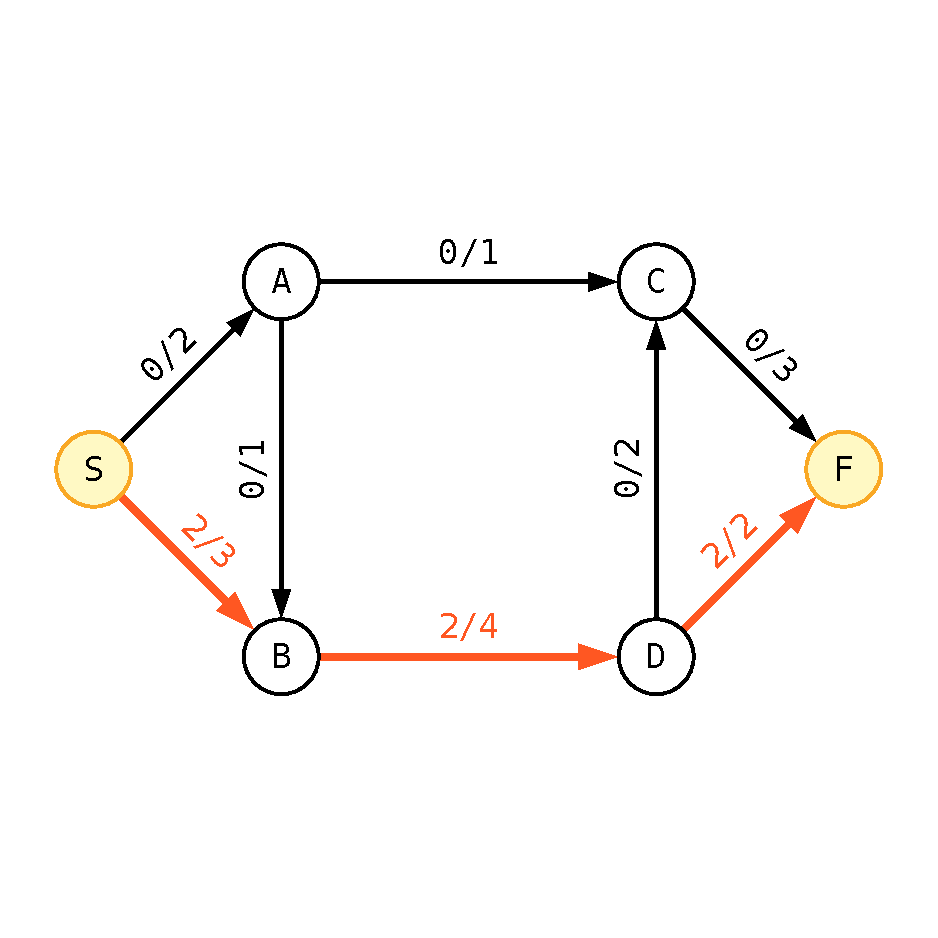
\includegraphics[width=0.46\textwidth]{python/lec09/flowexample/flowex-1.pdf}\\[2pt]{\scriptsize Путь 1: $S{,}B{,}D{,}F$, $\min = 2$, $|f| = 2$}} &
\shortstack{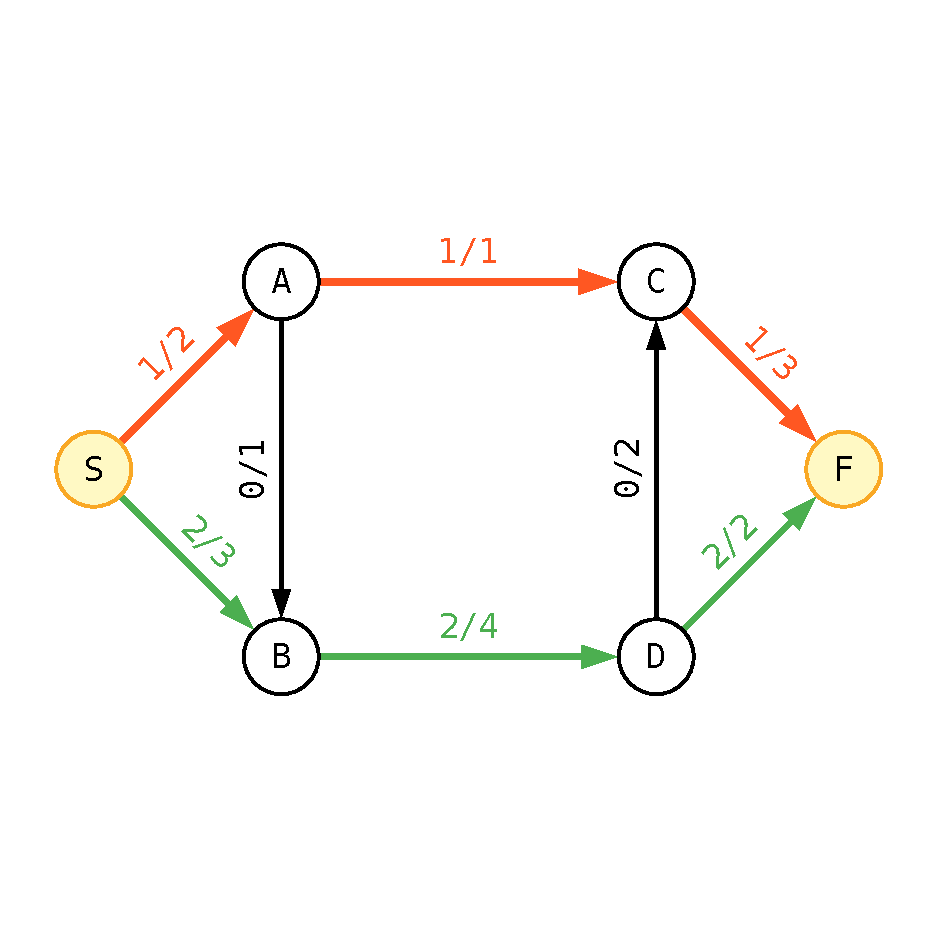
\includegraphics[width=0.46\textwidth]{python/lec09/flowexample/flowex-2.pdf}\\[2pt]{\scriptsize Путь 2: $S{,}A{,}C{,}F$, $\min = 1$, $|f| = 3$}} \\
\end{tabular}\end{center}
\begin{center}\begin{tabular}{cc}
\shortstack{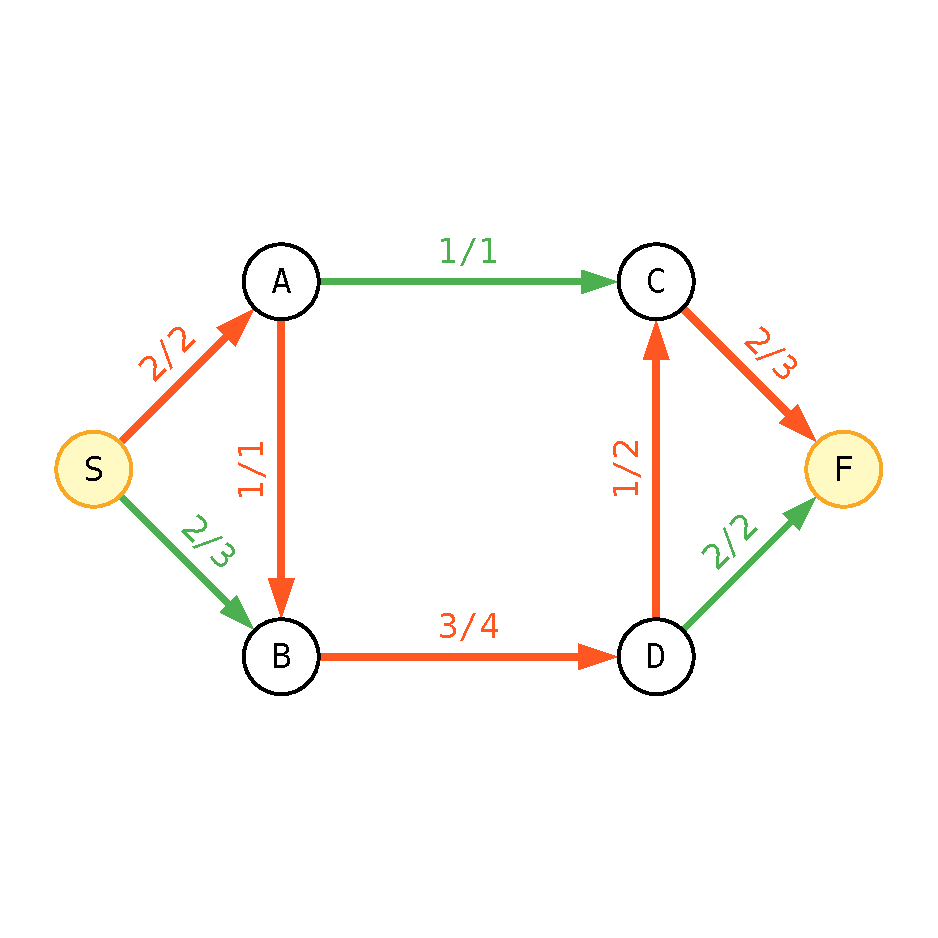
\includegraphics[width=0.46\textwidth]{python/lec09/flowexample/flowex-3.pdf}\\[2pt]{\scriptsize Путь 3: $S{,}A{,}B{,}D{,}C{,}F$, $\min = 1$, $|f| = 4$}} &
\shortstack{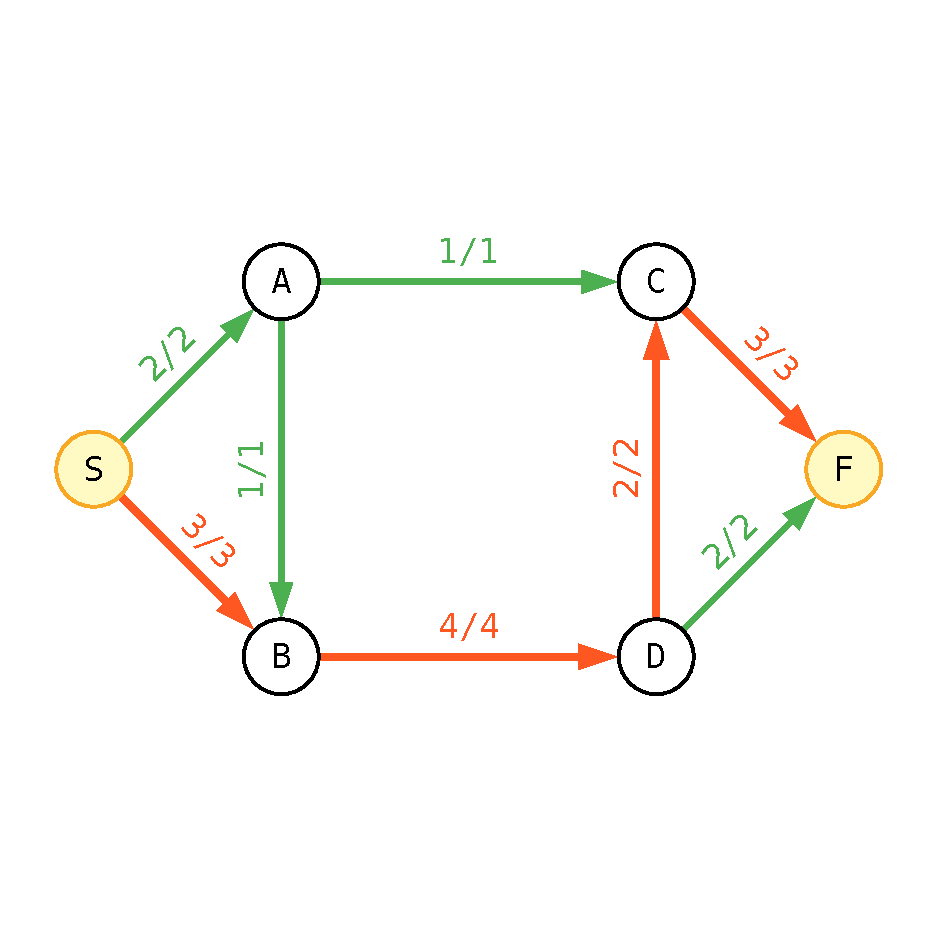
\includegraphics[width=0.46\textwidth]{python/lec09/flowexample/flowex-4.pdf}\\[2pt]{\scriptsize Путь 4: $S{,}B{,}D{,}C{,}F$, $\min = 1$, $|f| = 5$}} \\
\end{tabular}\end{center}
\begin{center}
\shortstack{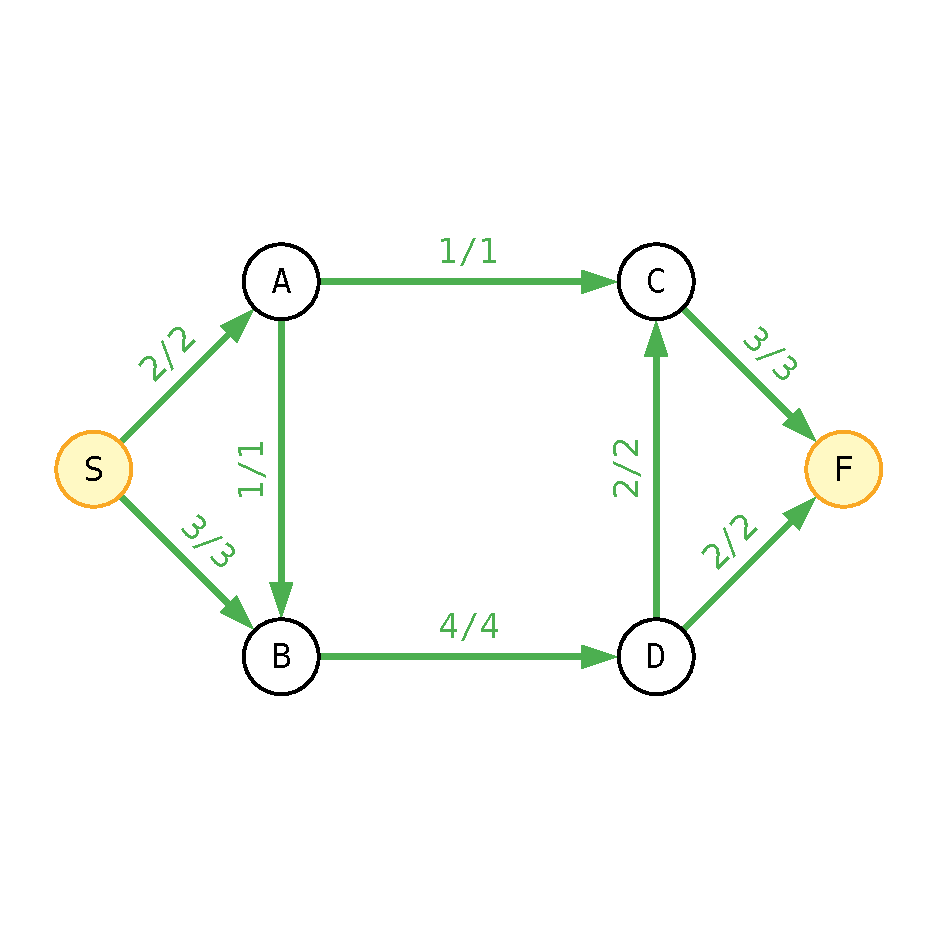
\includegraphics[width=0.5\textwidth]{python/lec09/flowexample/flowex-5.pdf}\\[2pt]{\scriptsize Итог: $|f| = 5$, оба ребра из $S$ насыщены}}
\end{center}

После каждого пути остаточные веса пересчитываются; при насыщении ребра
в общем случае добавляется фиктивное обратное ребро с остаточной
ёмкостью (подробно --- в лекции про алгоритм Форда--Фалкерсона).

\medskip
\textbf{Итог:}
условие балансировки выполняется в каждой внутренней вершине, и
$|f| = 2 + 1 + 1 + 1 = 5$ --- максимум: оба ребра из истока
($S{\to}A$ и $S{\to}B$) насыщены, больше из $S$ вытечь не может.

% ============================================================
\begin{task}{Наибольшее паросочетание в двудольном графе}{matching-task}
\textbf{Условие.} Дан двудольный граф с долями $\{a,b,c\}$ и $\{x,y,z\}$ и
рёбрами
\[
  a\!-\!x,\quad a\!-\!y,\quad b\!-\!x,\quad c\!-\!y,\quad c\!-\!z.
\]
Найдите наибольшее паросочетание (алгоритм Куна, поиск увеличивающих путей).

\begin{center}
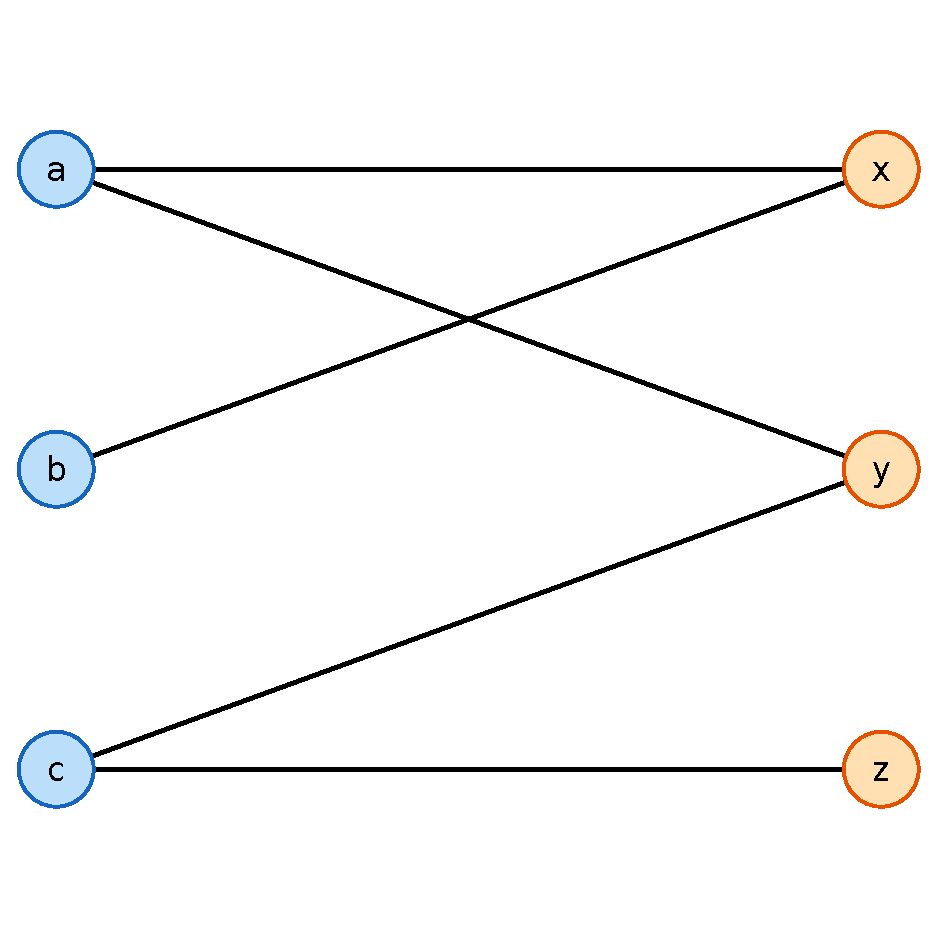
\includegraphics[width=0.4\textwidth]{figures/match-example.pdf}
\end{center}

\smallskip
\textbf{Решение.} Паросочетание --- набор попарно несмежных рёбер. Алгоритм Куна
по очереди пытается насытить каждую вершину левой доли, ища увеличивающий путь
(чередующий путь из свободной вершины в свободную).
\begin{enumerate}
  \item $a$: свободно ребро $a\!-\!x$ $\Rightarrow$ паросочетание $\{a\!-\!x\}$.
  \item $b$: единственное ребро $b\!-\!x$, но $x$ занят $a$. Ищем увеличивающий
        путь: $b\!-\!x$, $x$ занят $a$, у $a$ есть альтернатива $a\!-\!y$ ($y$
        свободна). Перекладываем: $a\!-\!y,\ b\!-\!x$. Паросочетание
        $\{a\!-\!y,\ b\!-\!x\}$.
  \item $c$: ребро $c\!-\!y$ ведёт к занятому $y$; пробуем $c\!-\!z$ ($z$
        свободна) $\Rightarrow$ добавляем $c\!-\!z$. Паросочетание
        $\{a\!-\!y,\ b\!-\!x,\ c\!-\!z\}$.
\end{enumerate}
Все три вершины левой доли насыщены --- паросочетание совершенное, его размер
$3$ (больше быть не может, так как доли по $3$ вершины).

\begin{center}
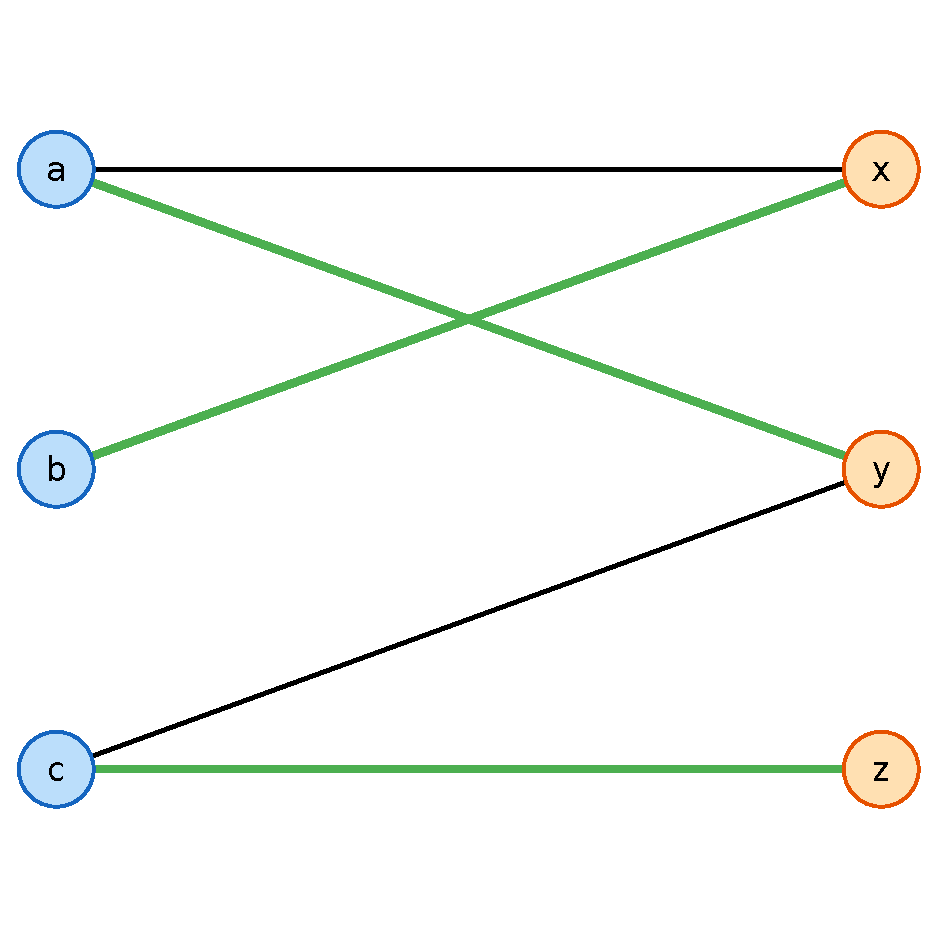
\includegraphics[width=0.4\textwidth]{figures/task-matching-sol.pdf}
\end{center}

\textbf{Ответ.} Наибольшее паросочетание: $\{a\!-\!y,\ b\!-\!x,\ c\!-\!z\}$,
размер $3$ (совершенное).
\end{task}
